% Created 2015-02-20 Пт 17:39
\documentclass[presentation]{beamer}

\usepackage[utf8]{inputenc}
\usepackage[T1]{fontenc}
\usepackage{fixltx2e}
\usepackage{graphicx}
\usepackage{longtable}
\usepackage{float}
\usepackage{wrapfig}
\usepackage{rotating}
\usepackage[normalem]{ulem}
\usepackage{amsmath}
\usepackage{textcomp}
\usepackage{marvosym}
\usepackage{wasysym}
\usepackage{amssymb}
\usepackage{hyperref}
\tolerance=1000
\usepackage[english, russian]{babel}
\usepackage[labelformat=empty]{caption}
\usepackage{subcaption}

\graphicspath{{graphics/}}

\usetheme[height=20pt]{Rochester}

\author{Артём Попцов}
\date{2015-04-26}

\title{Хакерспейсы}

\begin{document}
\maketitle

\begin{frame}{Содержание}

\setcounter{tocdepth}{1}
\tableofcontents
\end{frame}

\section{Что такое хакерспейс?}

\label{sec-1}
\subsection{Что такое хакерспейс?}

\label{sec-1-1}

\begin{frame}[label=sec-1-1-1]{Что такое хакерспейс?}
  \begin{columns}
    \begin{column}{0.5\textwidth}
      \begin{itemize}
      \item \alert{Физическое место}, где можно поработать
      \item \alert{Сообщество}, где можно найти поддержку
      \item \alert{Инструменты} для выполнения работ различного рода
      \end{itemize}
    \end{column}

    \begin{column}{0.5\textwidth}
      \begin{figure}[r]
        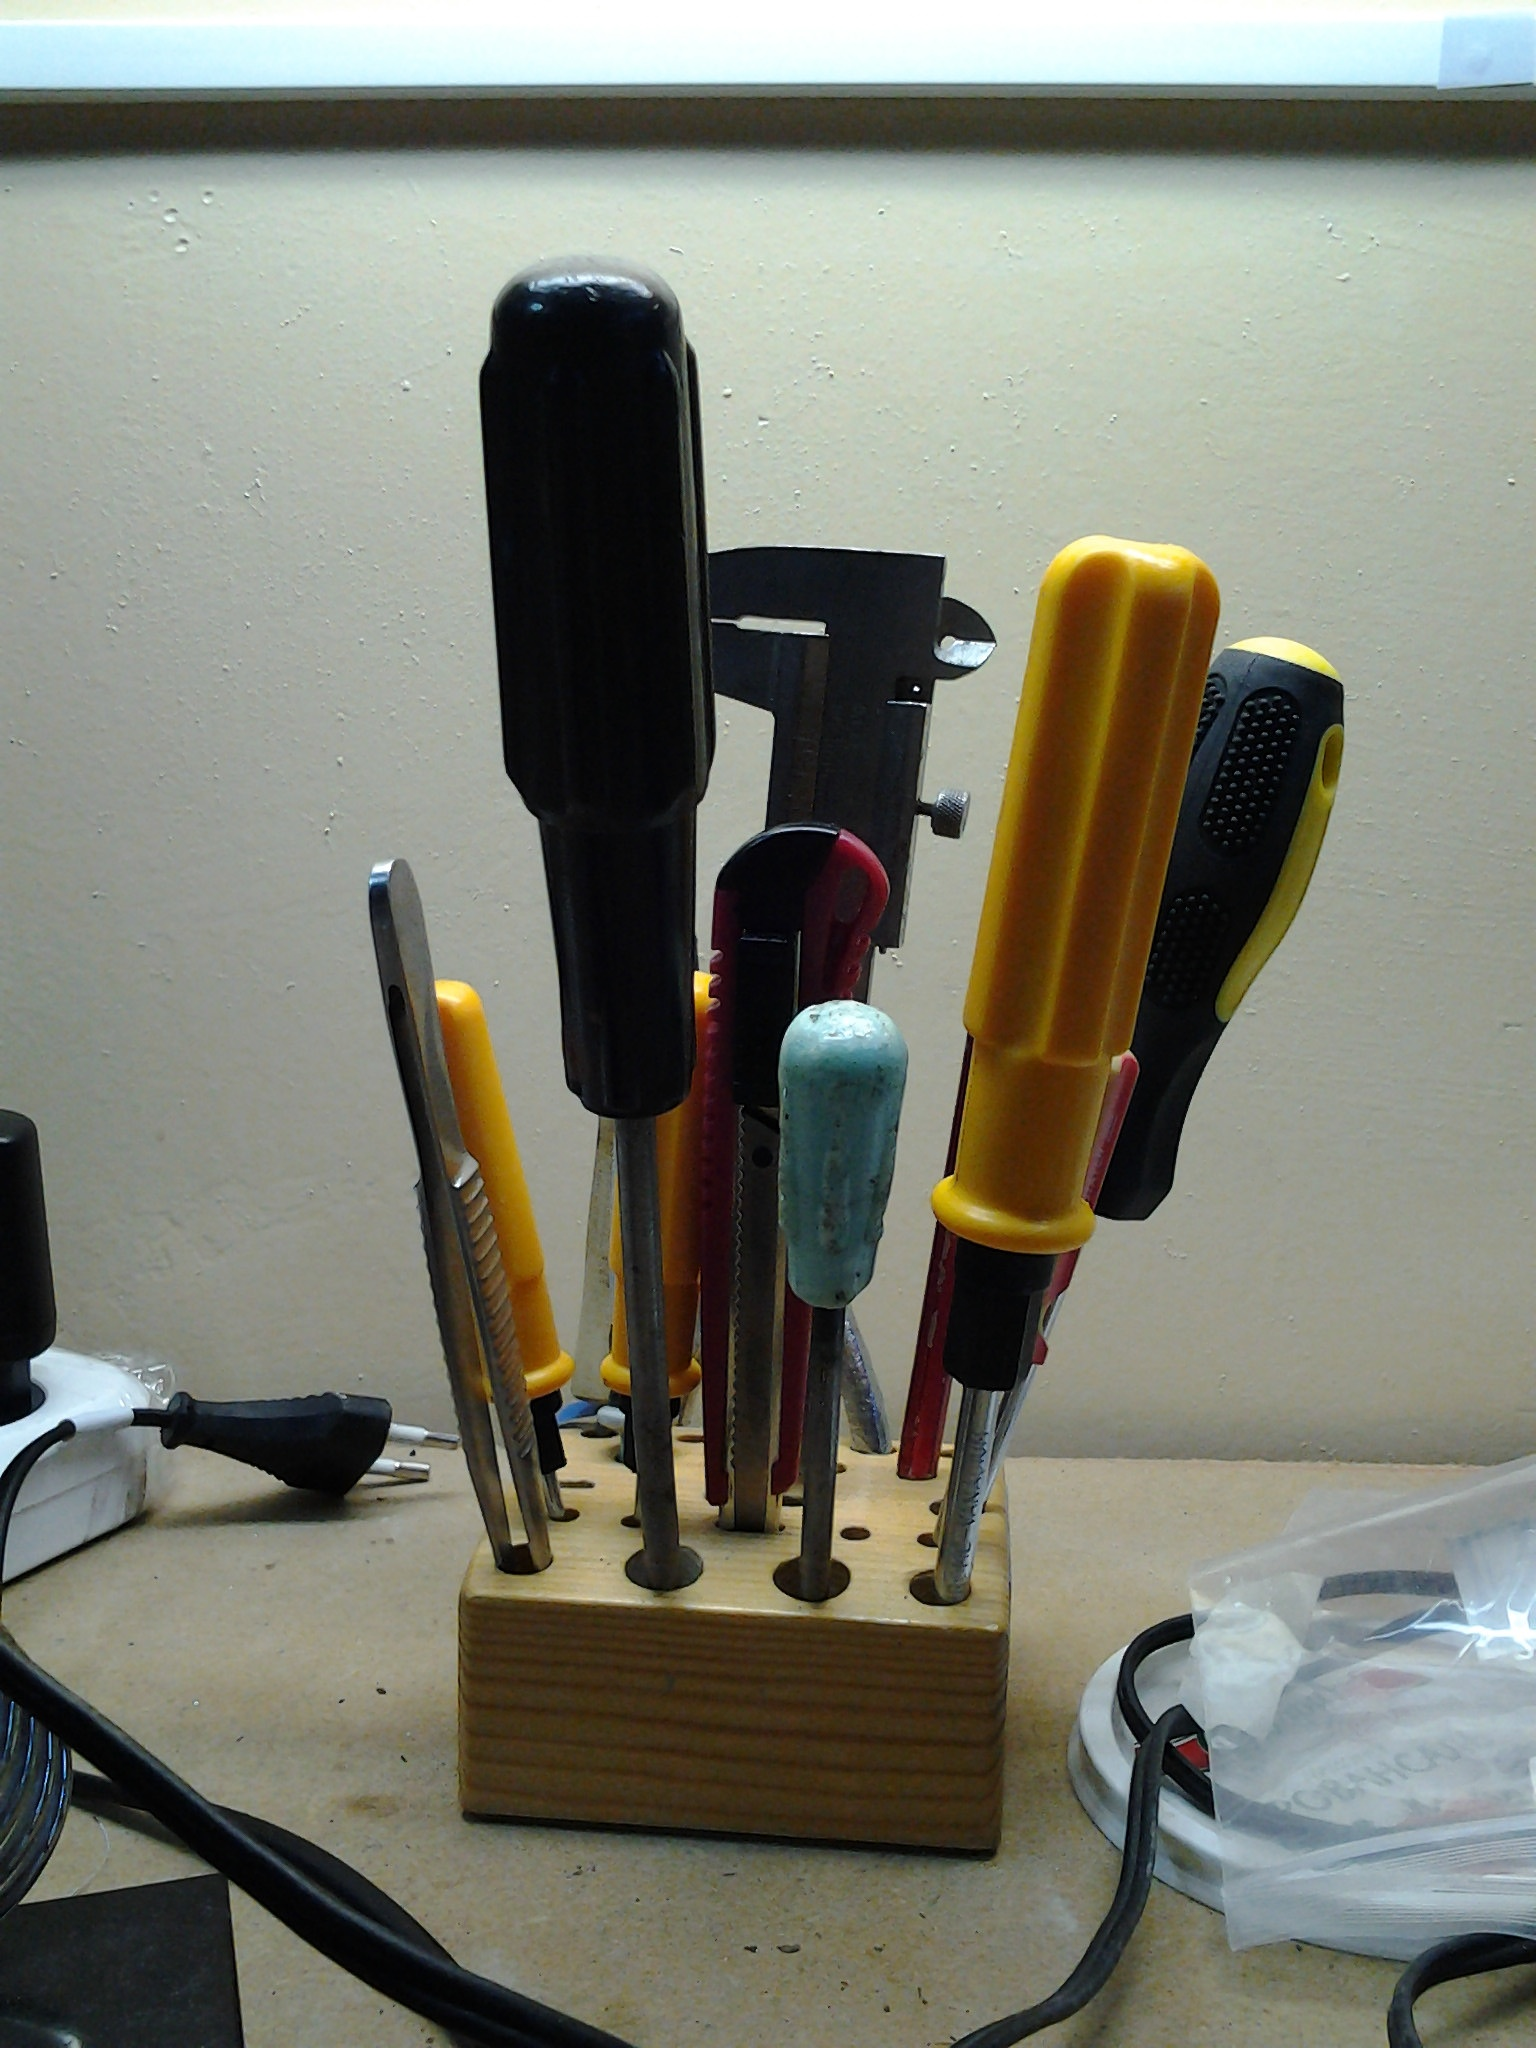
\includegraphics[width=.9\textwidth]{IMG_20150424_185329}
      \end{figure}
    \end{column}
  \end{columns}
\end{frame}

\subsection{Для чего нужен хакерспейс?}

\label{sec-1-2}
\begin{frame}[label=sec-1-2-1]{Для чего нужен хакерспейс?}
  \begin{columns}
    \begin{column}{0.5\textwidth}
      \begin{itemize}
      \item \alert{Работа} над проектами
      \item \alert{Общение}, "подзарядка идеями"
      \item \alert{Творчество} и возможность самовыражения
      \item \alert{Обучение} на практике
      \end{itemize}
    \end{column}
    \begin{column}{0.5\textwidth}
      \begin{figure}[r]
        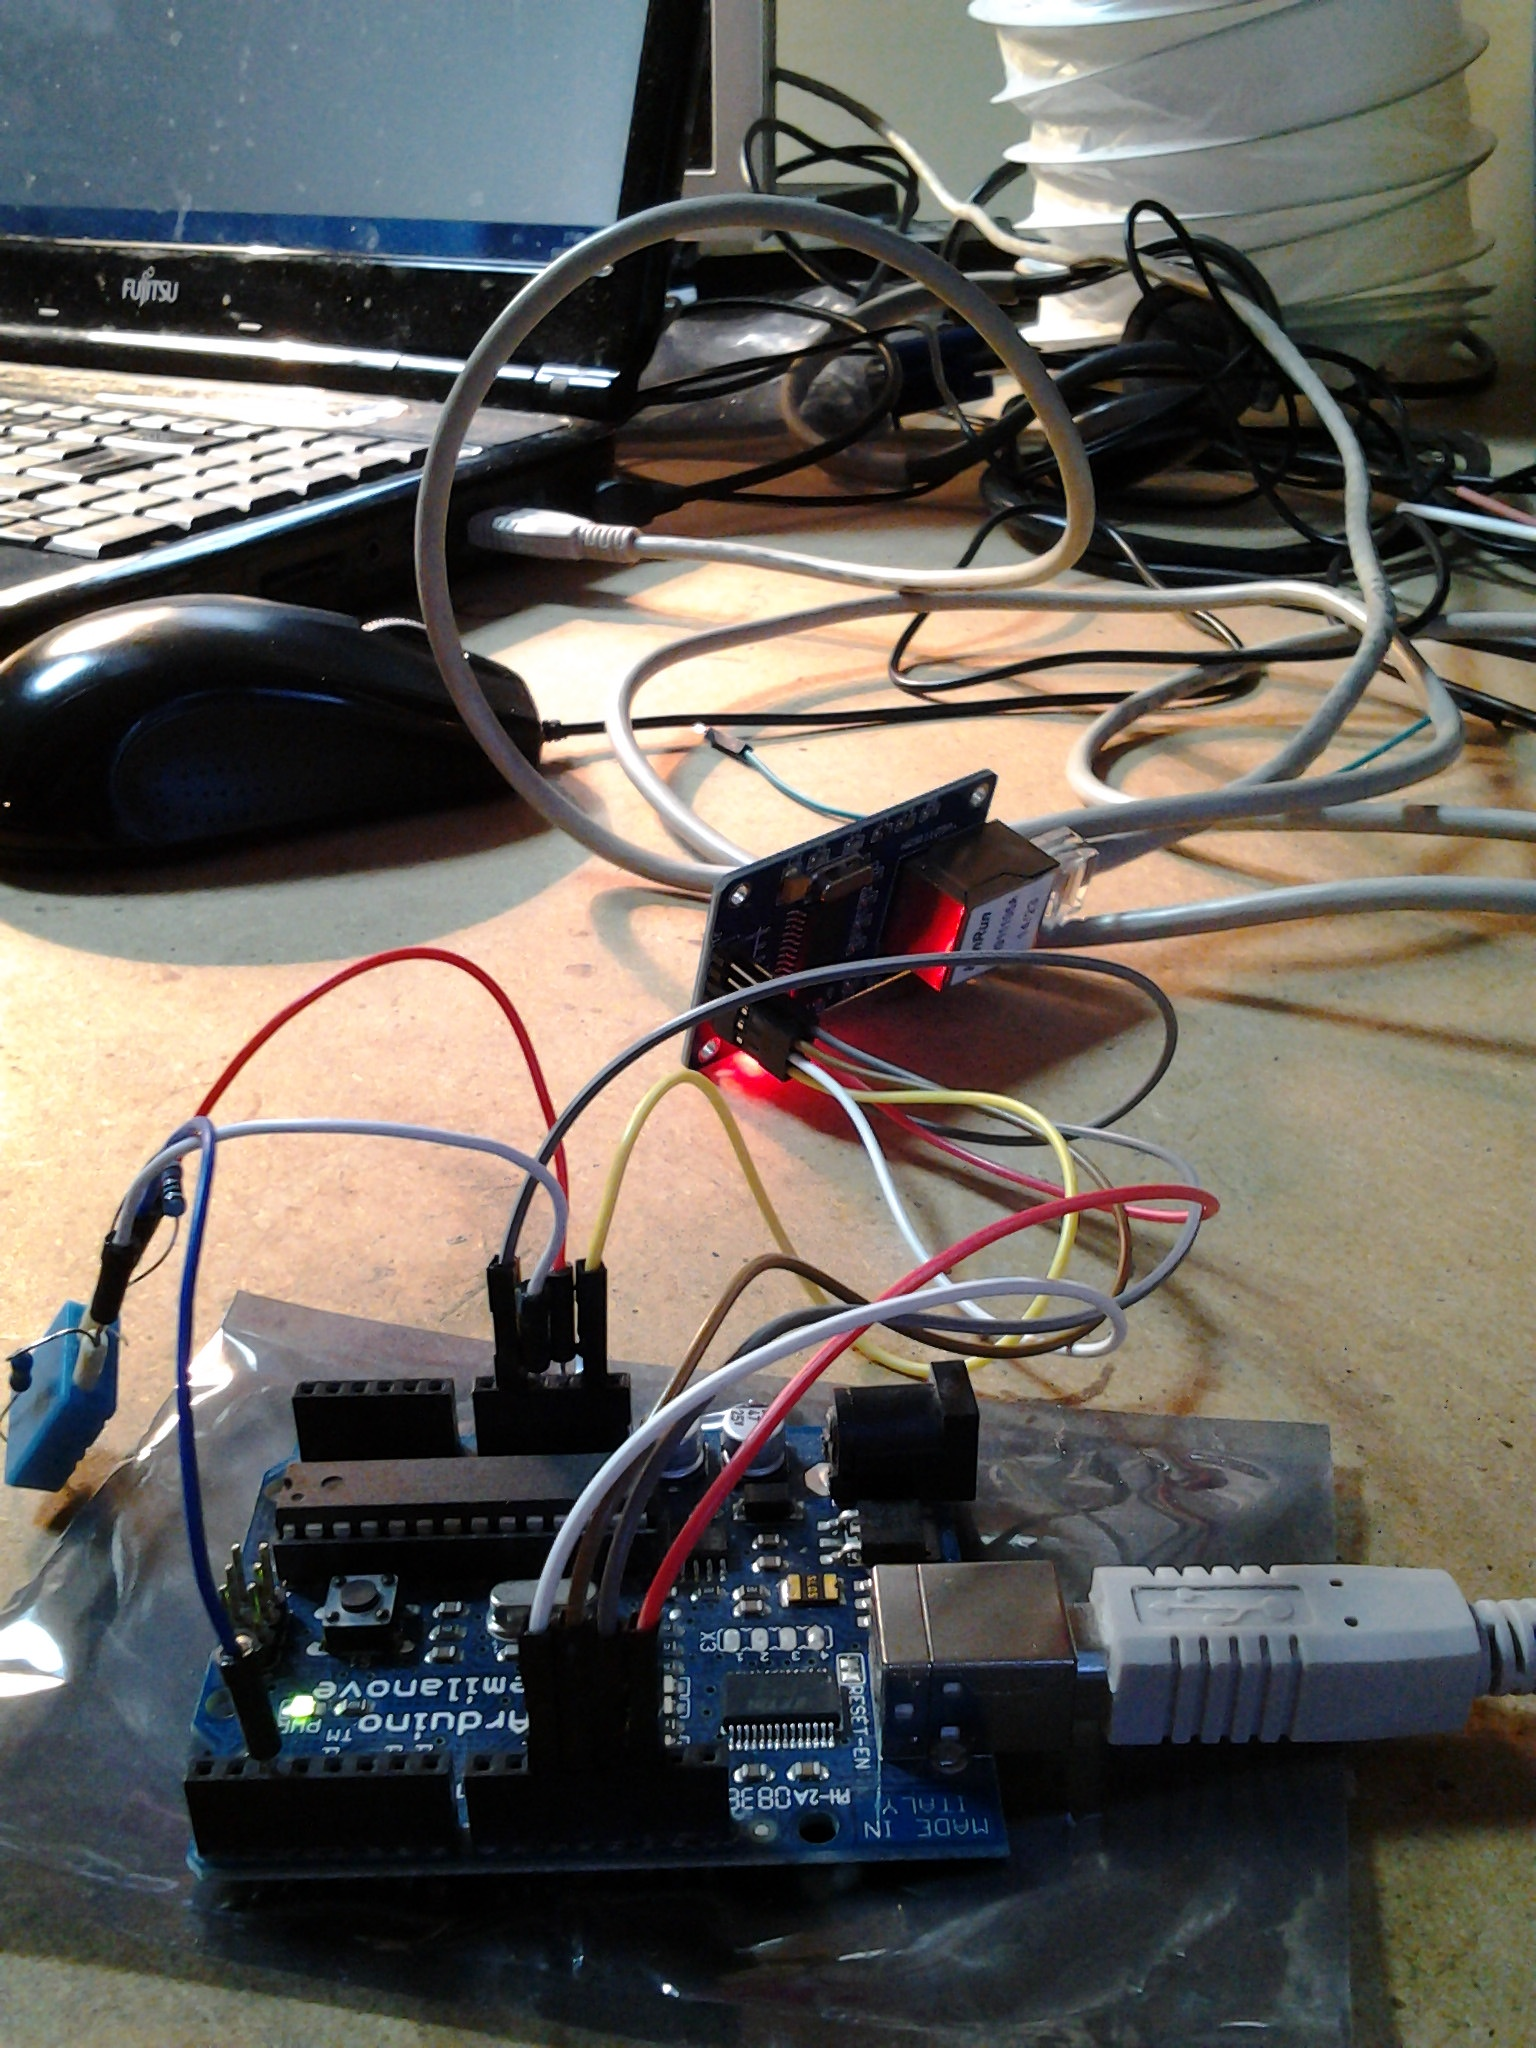
\includegraphics[width=.9\textwidth]{IMG_20150307_174539}
      \end{figure}
    \end{column}
  \end{columns}
\end{frame}

\section{Хакерспейсы в мире}

\subsection{Хакерспейсы в мире}

\begin{frame}[label=1-3-1]{Хакерспейсы в мире}
  Некоторые факты:
  \begin{itemize}
    \item Первые хакерспейсы начали создаваться в 90-х годах.
    \item \alert{более 1150} активных хакерспейсов по всему миру (на
      2015-04-25).
  \end{itemize}
  \begin{figure}[htb]
    \centering
    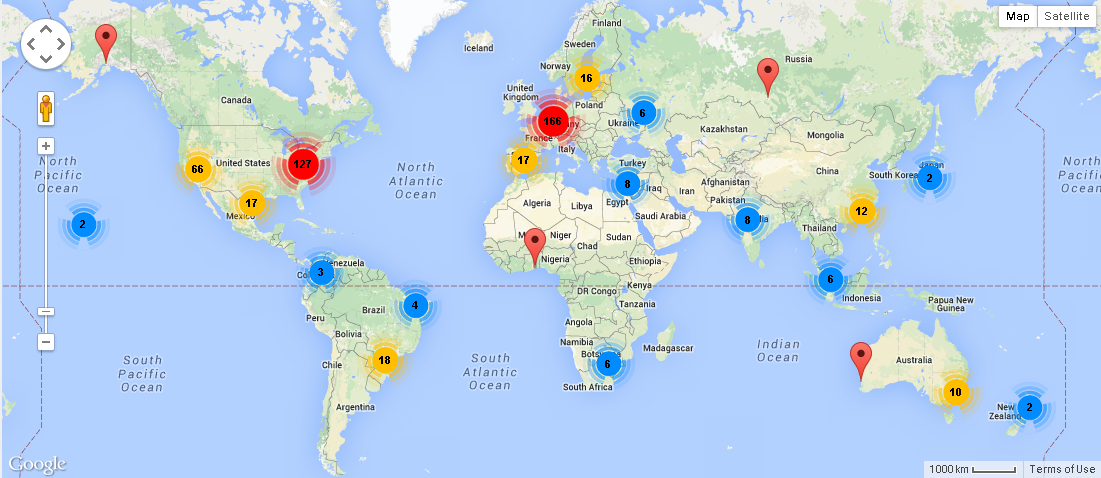
\includegraphics[width=.9\linewidth]{active-hackerspaces-2015-04-25}
    \caption{Активные хакерспейсы (источник: hackerspaces.org)}
  \end{figure}
\end{frame}

\begin{frame}[label=1-3-2]{Хакерспейсы в мире}
  Примеры:
  \begin{columns}
    \begin{column}{0.5\textwidth}
      \begin{itemize}
      \item c-base (Germany)
      \item Metalab (Austria)
      \item Noisebridge (USA)
      \item NYC Resistor (USA)
      \item Pumping Station: One (USA)
      \end{itemize}
    \end{column}
    \begin{column}{0.5\textwidth}
      \begin{itemize}
      \item RaumZeitLabor (Germany)
      \item syn2cat (Germany)
      \item Neúron (Russia)
      \item SZDIY (China)
      \end{itemize}
    \end{column}
  \end{columns}
  \begin{figure}[htb]
    \centering
    
\includegraphics[width=.9\linewidth]{hackerspace-logos}
  \end{figure}
\end{frame}

\label{sec-1-3}
\begin{frame}[label=sec-1-3-3]{hackerspaces.org}
  \begin{columns}
    \begin{column}{0.4\textwidth}
      \begin{itemize}
      \item Каталог хакерспейсов
      \item События
      \item Документация
      \item Проекты
      \item Список людей
      \item Список образовательных ресурсов
      \item Информация о ПО/аппаратном обеспечении
      \item \ldots
      \end{itemize}
    \end{column}
    \begin{column}{0.6\textwidth}
    \begin{figure}[htb]
      \centering
      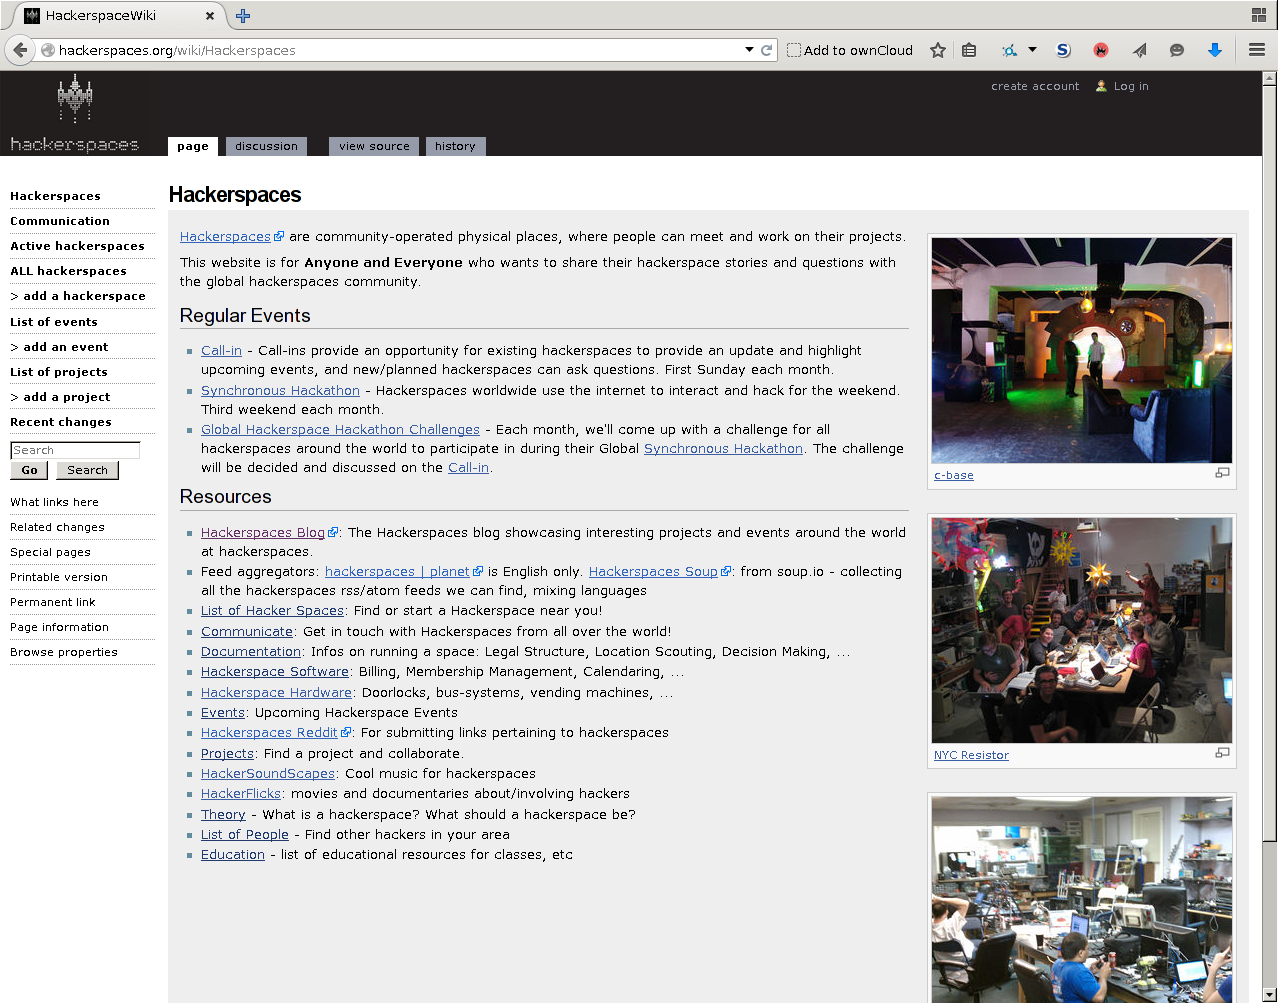
\includegraphics[width=.9\linewidth]{hackerspaces-org}
      \caption{\label{hackerspaces-org}Wiki на hackerspaces.org}
    \end{figure}
    \end{column}
  \end{columns}
\end{frame}

\section{Хакерспейсы в России}
\subsection{Хакерспейсы в России}

\begin{frame}[label=sec-1-3-4]{Хакерспейсы в России}
  \begin{figure}[htb]
    \centering
    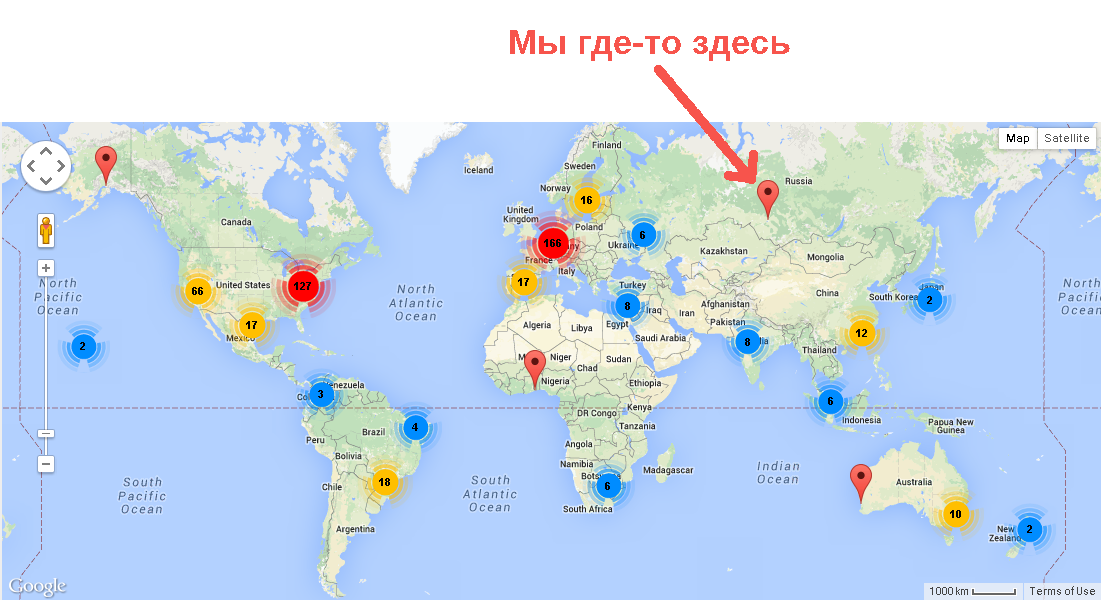
\includegraphics[width=1\linewidth]{active-hackerspaces-2015-04-25-w-arrow}
    \caption{Привет, мир!}
  \end{figure}
\end{frame}

\begin{frame}[label=sec-1-3-5]{Хакерспейсы в России}
  \begin{figure}[htb]
    \centering
    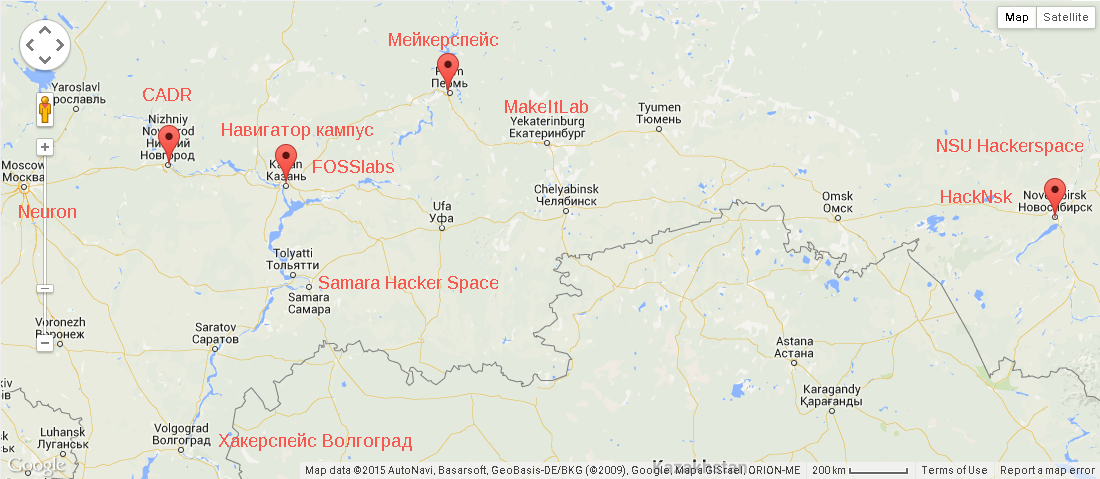
\includegraphics[width=1\linewidth]{active-hackerspaces-russia-2015-04-25}
    \caption{\label{active-hackerspaces-russia}Хакерспейсы на
      территории России (2015-04-25)}
  \end{figure}
\end{frame}

\begin{frame}[label=sec-1-3-6]{Хакерспейсы в России}
  \begin{columns}
    \begin{column}{0.3\textwidth}
      \begin{figure}[htb]
        \includegraphics[width=\linewidth]{logos/HackSpace.jpg}
      \end{figure}
    \end{column}
    \begin{column}{0.7\textwidth}
      \begin{itemize}
      \item Хакерспейс HackSpace в Таганроге
      \item Находится в одном из корпусов Южного федерального
        университета
      \item Предоставляют 3D-принтер, 3D-сканер, одноплатные ПК,
        Arduino, паяльные станции и пр.
      \end{itemize}
    \end{column}
  \end{columns}
  \centering
  \vspace{5em}
  ictis.sfedu.ru/hackspace
\end{frame}

\section{Нижегородский хакерспейс CADR}

\label{sec-2}
\subsection{Нижегородский хакерспейс CADR}

\label{sec-2-1}
\begin{frame}[label=sec-2-1-1]{Нижегородский хакерспейс CADR}
  \begin{figure}[htb]
    
\includegraphics[width=.3\linewidth]{cadr-logo}
  \end{figure}

  \begin{itemize}
  \item Помещение 18 м$^{\text{2}}$, предоставленное Нижегородским
    Радиотехническим Колледжем (аудитория 054).
  \item Бесплатный доступ в помещение и к оборудованию хакерспейса
  \item Электричество, проводной/беспроводной интернет, чай/печеньки
  \end{itemize}
\end{frame}

\begin{frame}[label=sec-2-1-2]{Оборудование}
  \begin{figure}[htb]
    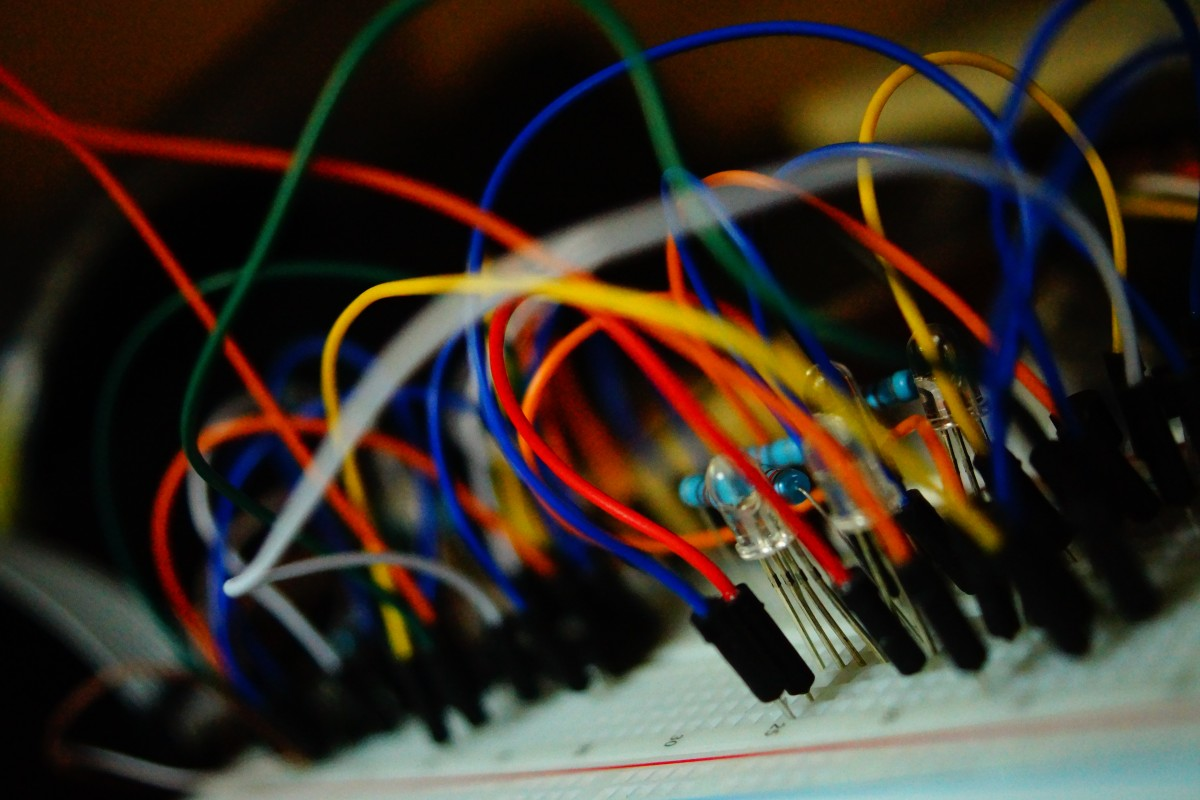
\includegraphics[
      width=.6\linewidth,
      clip,
      trim=0mm 20mm 0mm 50mm
    ]{DSC09211-1200x800}
  \end{figure}
  \vspace{-1em}
  \begin{columns}
    \begin{column}{0.5\textwidth}
      \small
      \begin{itemize}
      \item 3D-принтер
      \item Обычные принтеры (лазерный, матричный)
      \item Несколько ПК, ноутбук, периферия
      \item Web-камеры разных сортов
      \item Осциллограф, паяльник
      \item Монтажные платы
      \end{itemize}
    \end{column}
    \begin{column}{0.5\textwidth}
      \small
      \begin{itemize}
      \item Отвёртки, пассатижи, плоскогубцы, узкогубцы, \ldots
      \item Одноплатные компьютеры (Raspberry Pi, Hackberry, Intel
        Galileo, Intel Edison)
      \item Оборудование для ЛУТ
      \item Электронная ``рассыпуха'' \textit{почти} на все случаи
        жизни
      \item \ldots
      \end{itemize}
    \end{column}
  \end{columns}
\end{frame}

\begin{frame}[label=sec-2-1-2]{Помещение}
  \begin{columns}
    \begin{column}{0.5\textwidth}
      \begin{figure}
        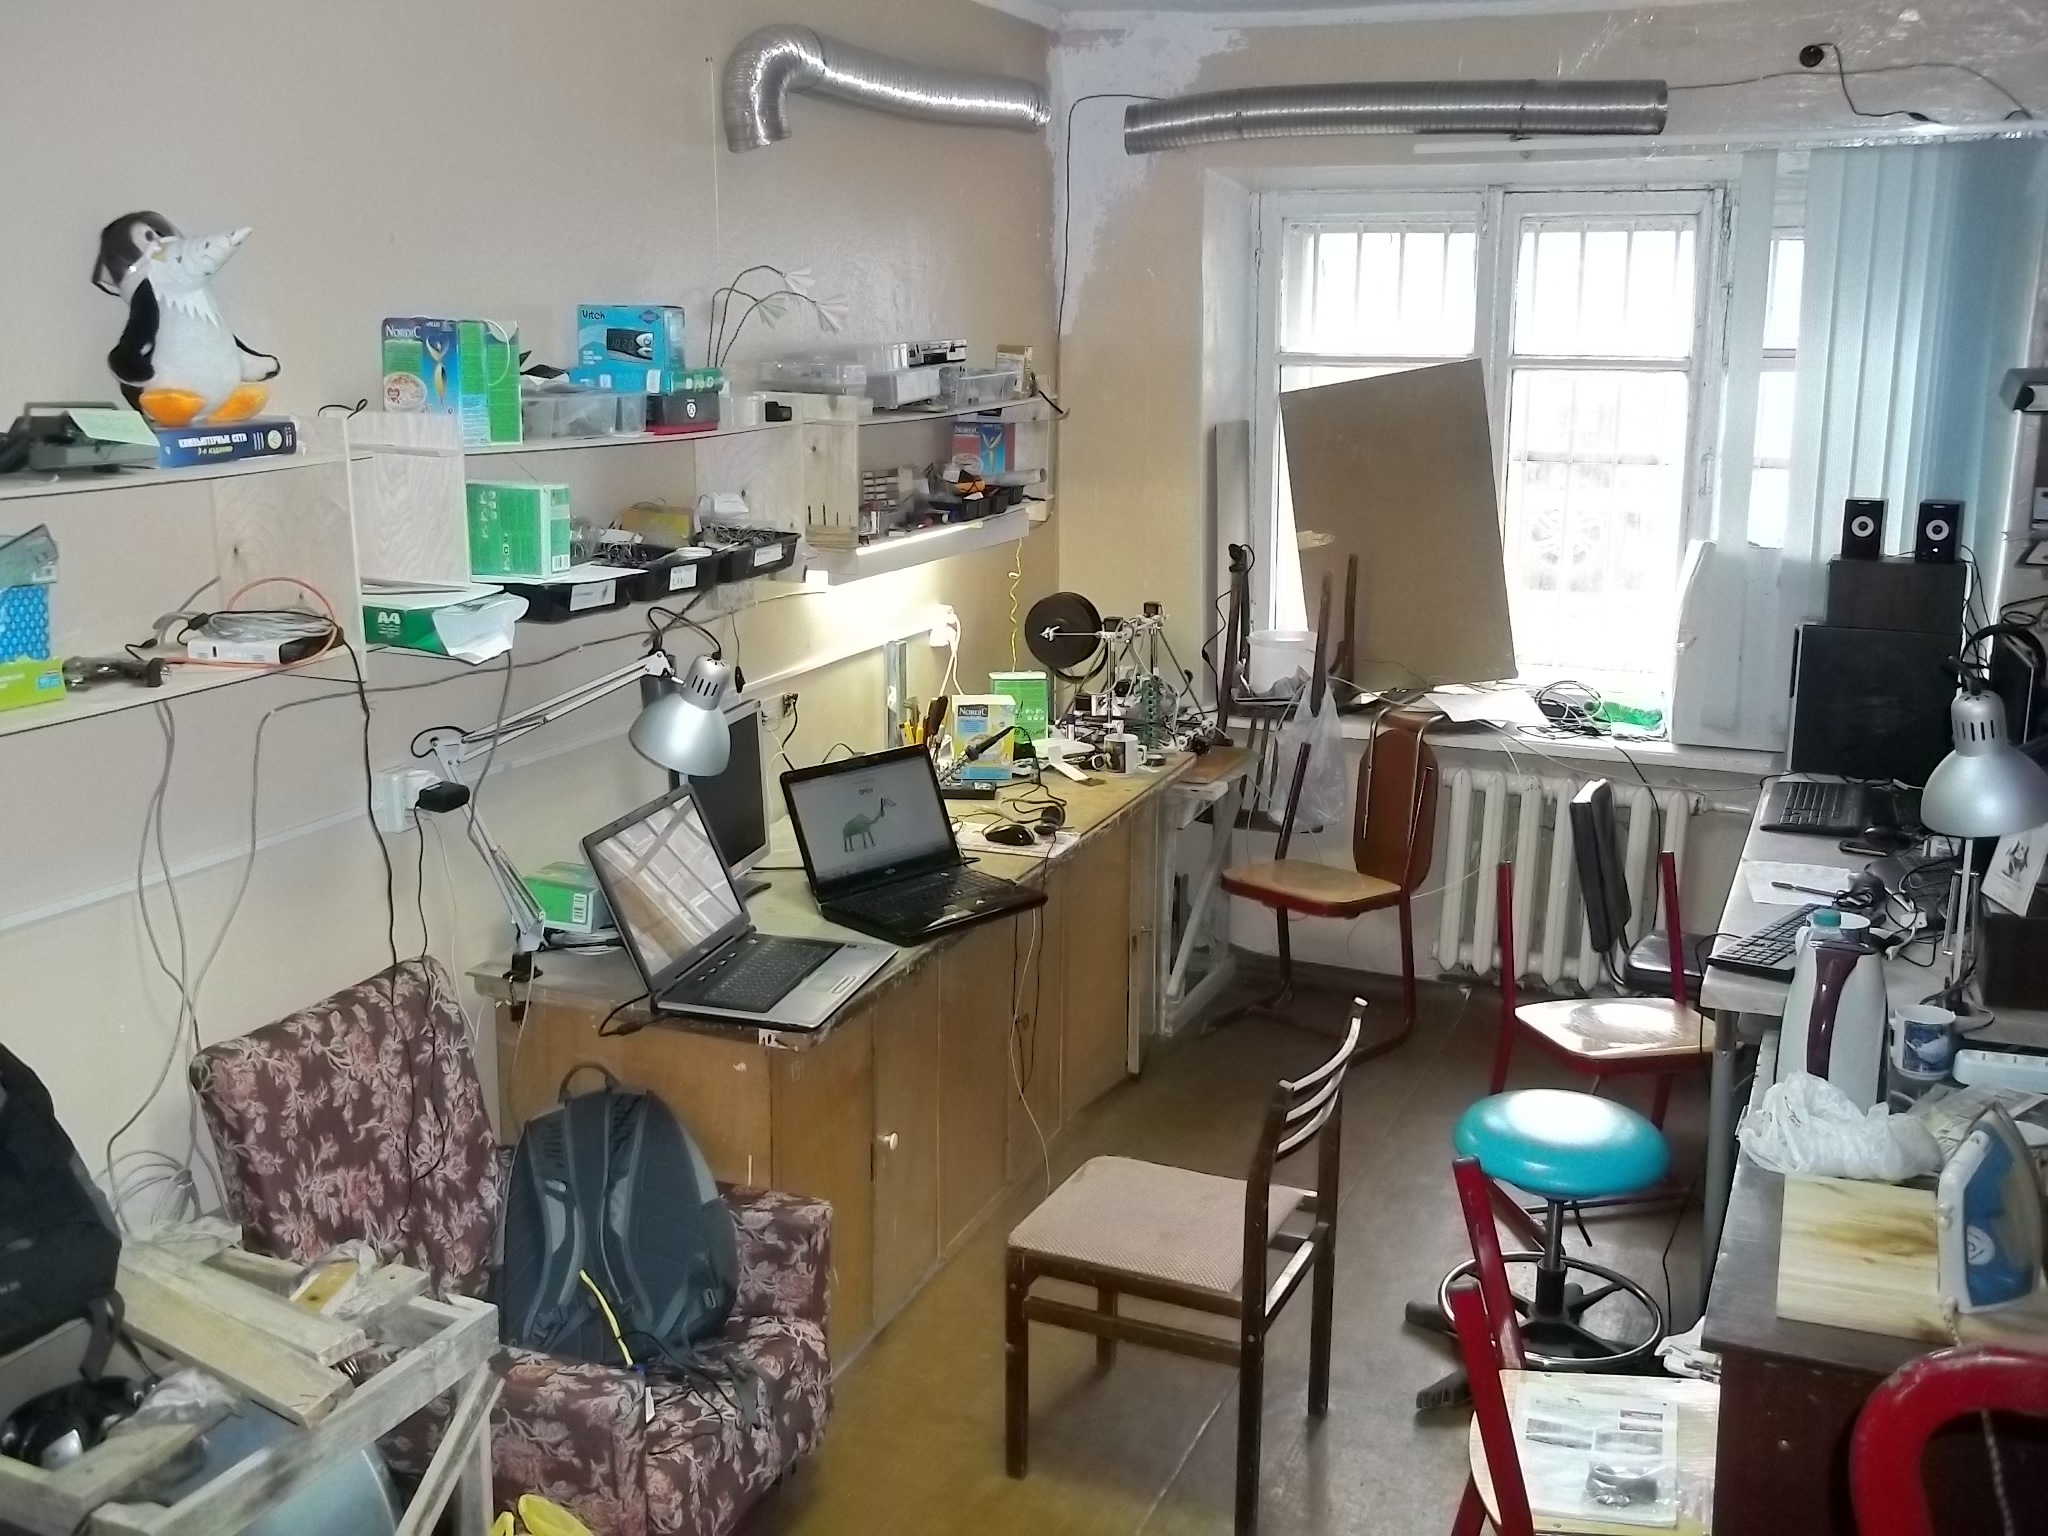
\includegraphics[width=\linewidth]{cadr-room-1.jpg}
        \caption{Монтажно-компьтерная зона}
      \end{figure}
    \end{column}
    \begin{column}{0.5\textwidth}
      \begin{figure}
        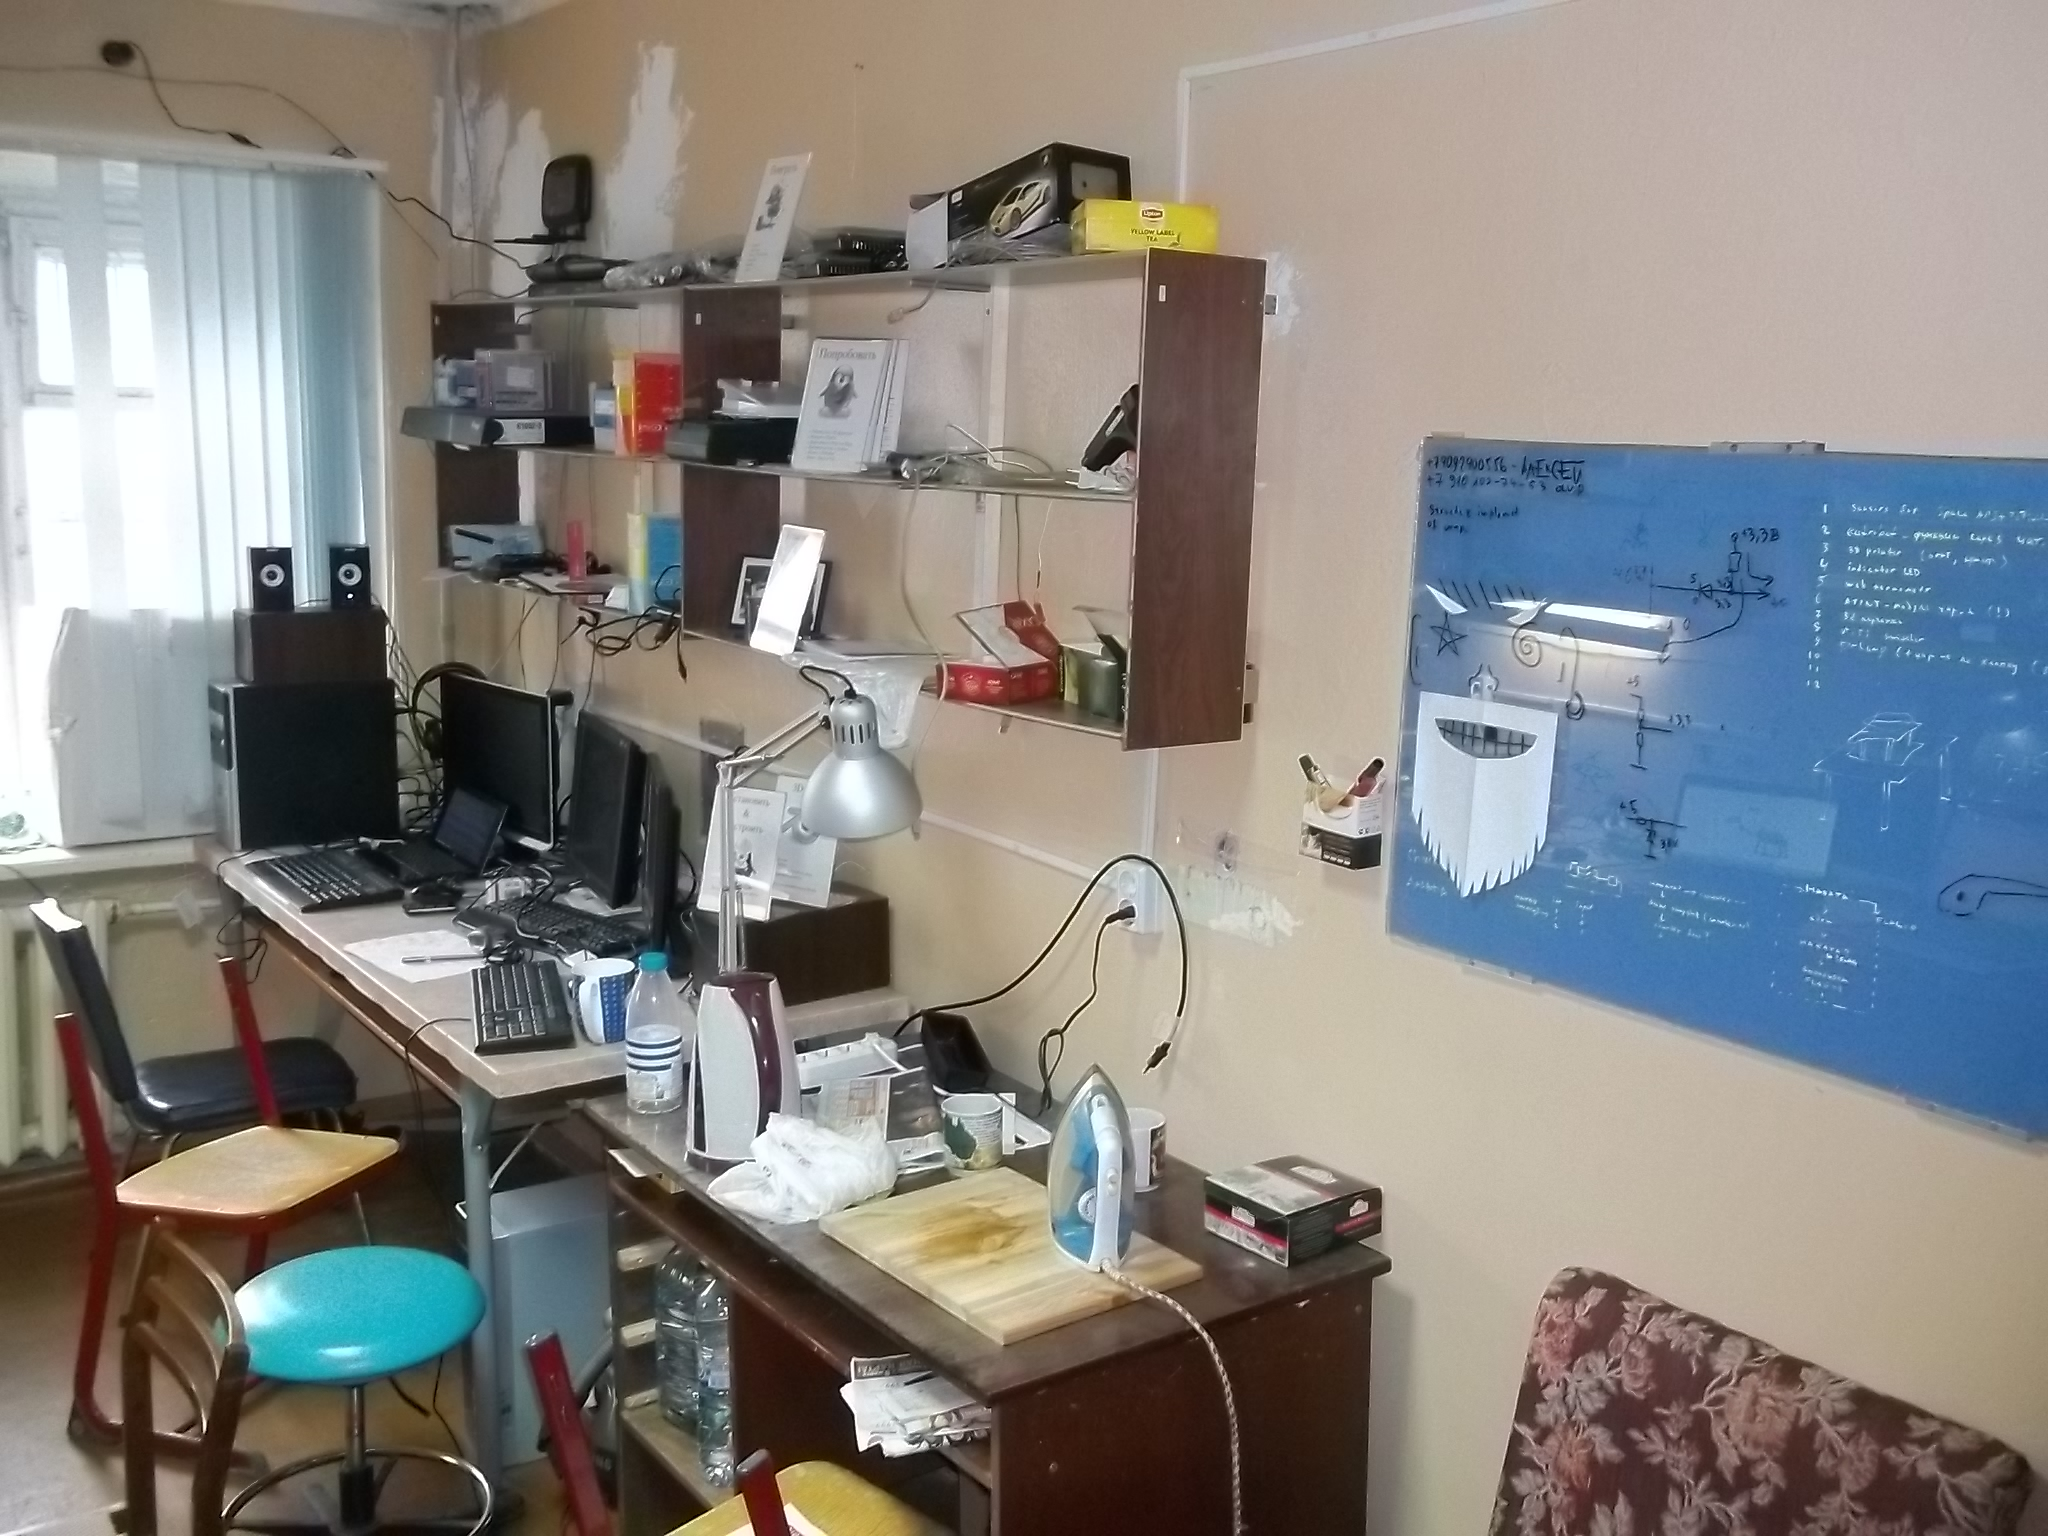
\includegraphics[width=\linewidth]{cadr-room-2.jpg}
        \caption{Компьютерно-монтажная зона}
      \end{figure}
    \end{column}
  \end{columns}
\end{frame}

\subsection{Чем мы занимаемся?}

\begin{frame}[label=sec-2-2-1]{Чем мы занимаемся?}
  \begin{itemize}
    \item Обмениваемся опытом -- учимся сами, помогаем учиться другим
    \item Проводим свободные лекции и участвуем в проведении
      конференций
    \item Работаем над несколькими проектами -- личными и совместными
  \end{itemize}
  \begin{figure}
    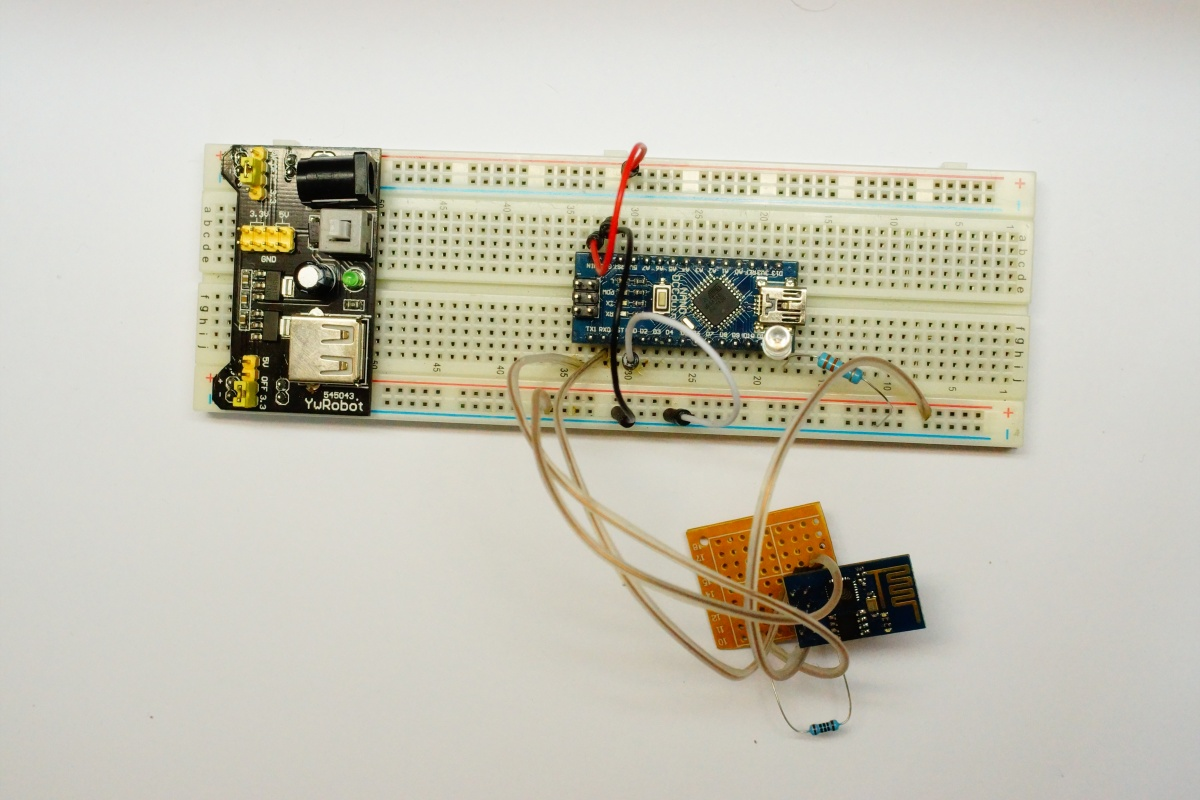
\includegraphics[
      width=.8\linewidth,
      clip,
      trim=0mm 0mm 0mm 30mm]{DSC09208-1200x800}
  \end{figure}
\end{frame}

\begin{frame}[label=sec-2-2-2]{Сборка 3D-принтера}
  \begin{itemize}
  \item Сборка из готовых частей и настройка
  \item Процесс подробно описан на сайте CADR'а
  \item Проект завершён успешно
  \end{itemize}
  \begin{figure}[htb]
    \centering
    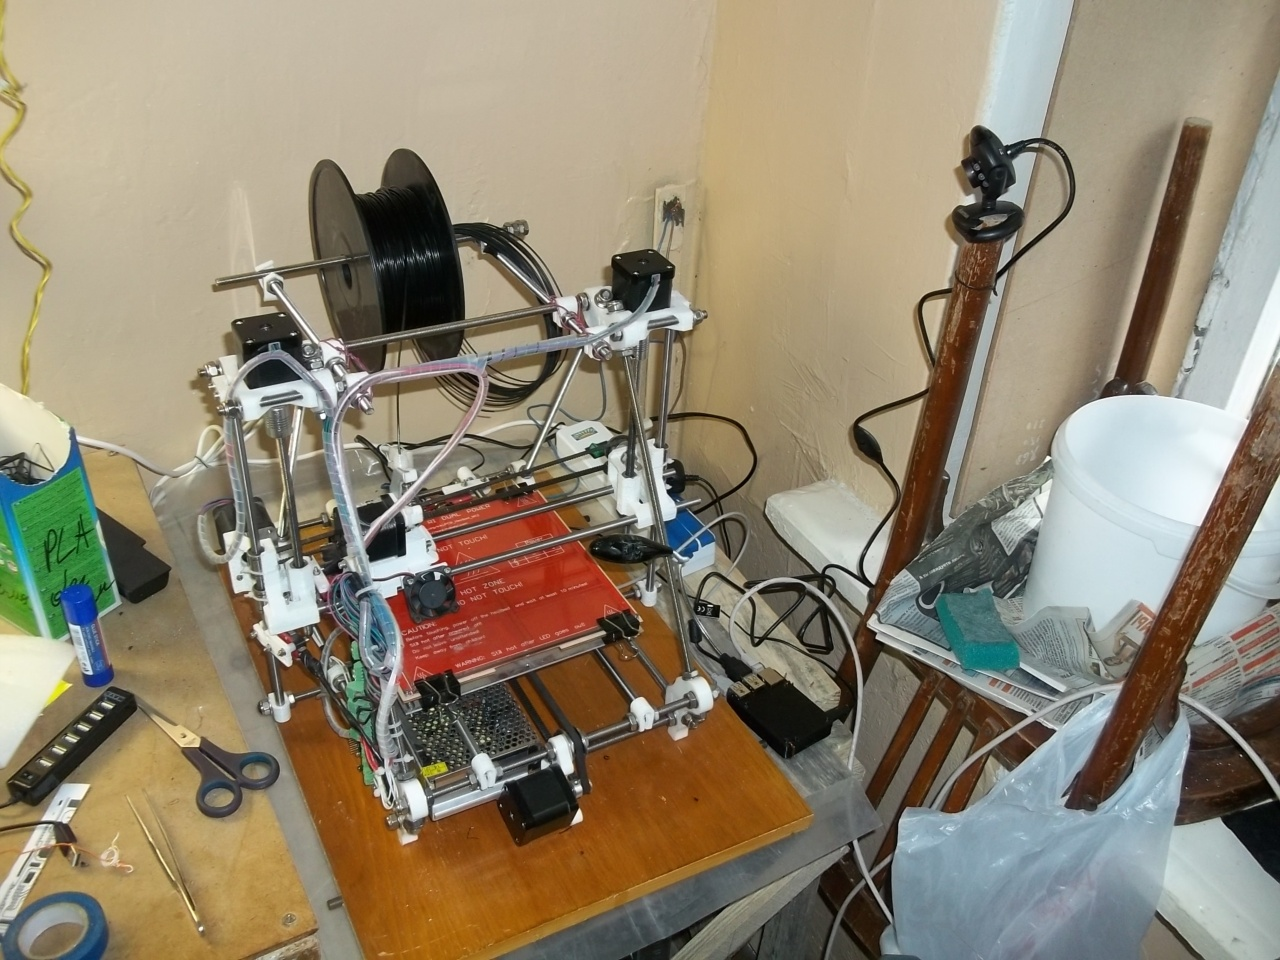
\includegraphics[
      width=.7\linewidth,
      clip,
      trim=20mm 20mm 70mm 40mm]{cadr-3d-printer}
    \caption{RepRap Mendel}
  \end{figure}
\end{frame}

\begin{frame}[label=sec-2-2-2]{Cisco + Raspberry Pi B + Asterisk}
  \begin{figure}[htb]
    \centering
    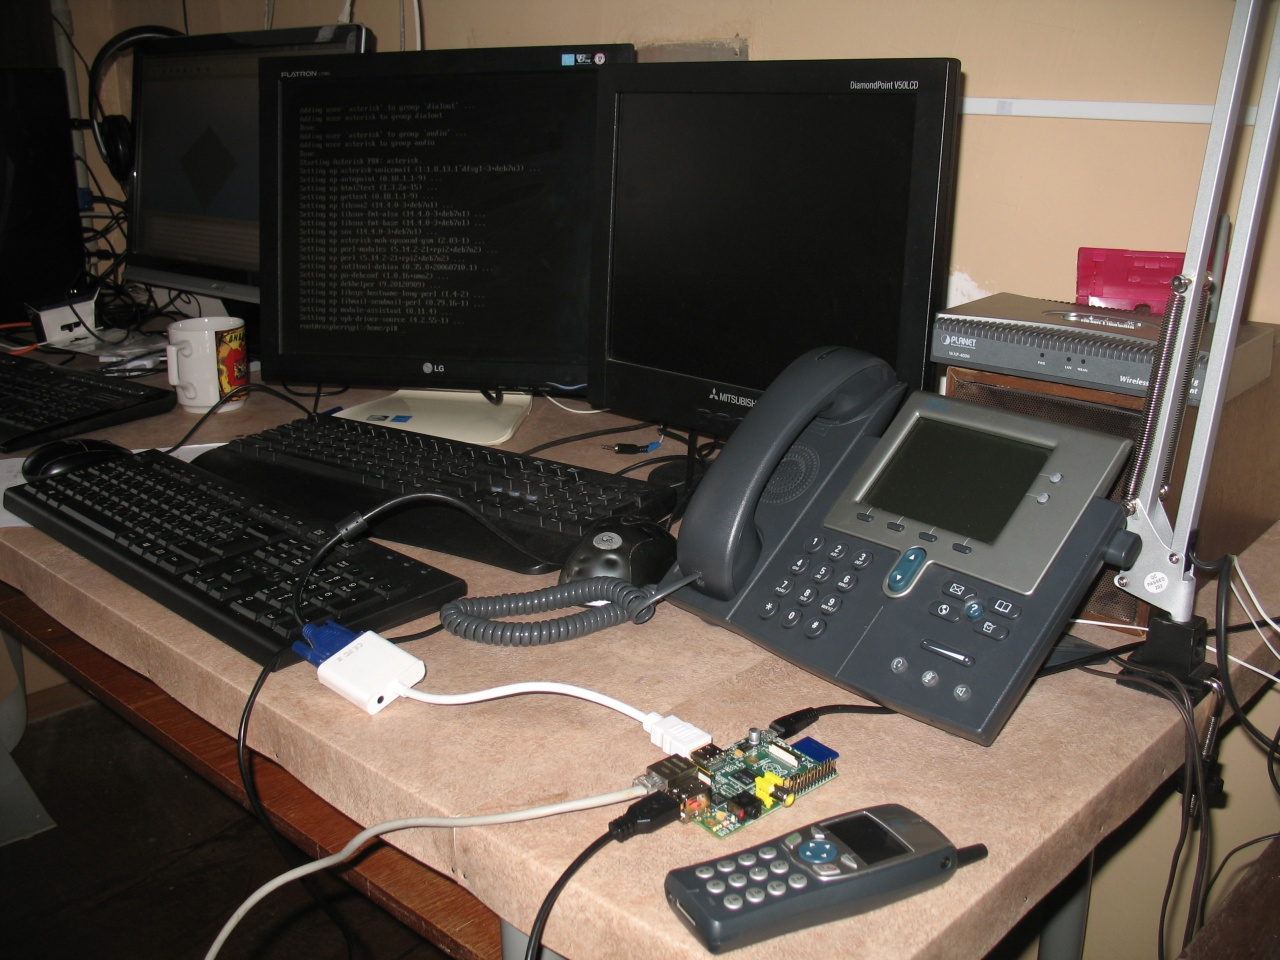
\includegraphics[width=.9\linewidth]{cadr-cisco-asterisk}
    \caption{Подключение оборудования Cisco 7920 и Cisco 7941 к
      Asterisk}
  \end{figure}
\end{frame}

\begin{frame}[label=sec-2-2-2]{Встречи для подписи ключей}
  \begin{figure}[htb]
    \centering
    
\includegraphics[width=.9\linewidth]{cadr-logo-crypto}
  \end{figure}
  \begin{itemize}
    \item В 2014-м году провели первую встречу для подписи GPG-ключей,
      совмещённую с конференцией по информационной безопасности от
      НРТК
    \item Планируем регулярно проводить аналогичные мероприятия
  \end{itemize}
\end{frame}

\begin{frame}[label=sec-2-2-2]{Подключение CADR'а к SpaceAPI}
  \begin{itemize}
  \item Осуществлено подключение хакерспейса к SpaceAPI (spaceapi.net)
    для отображения его статуса
  \item Подготовлена и записана на видео-лекция по данной теме
  \item Создан виджет для оконного менеджера Awesome, отображающий
    статус хакерспейса (github.com/artyom-poptsov/awesome\_space)
  \item Отображение статуса с помощью инновационной технологии
    (см. \textbf{cadrspace.ru/status})
  \end{itemize}
  \begin{figure}[htb]
    \centering
    
\includegraphics[width=.9\linewidth]{cadr-status}
  \end{figure}
\end{frame}

\begin{frame}[label=sec-2-2-3]{Исследование на тему интернета вещей}
  \begin{itemize}
    \item Подготовлена и записана лекция по фреймворку IoTivity
    \item Сделано несколько тестовых проектов
    \item Работаем над проектом, использующим фреймворк для сбора
      информации с датчиков в хакерспейсе
  \end{itemize}
  \begin{figure}[htb]
    \centering
    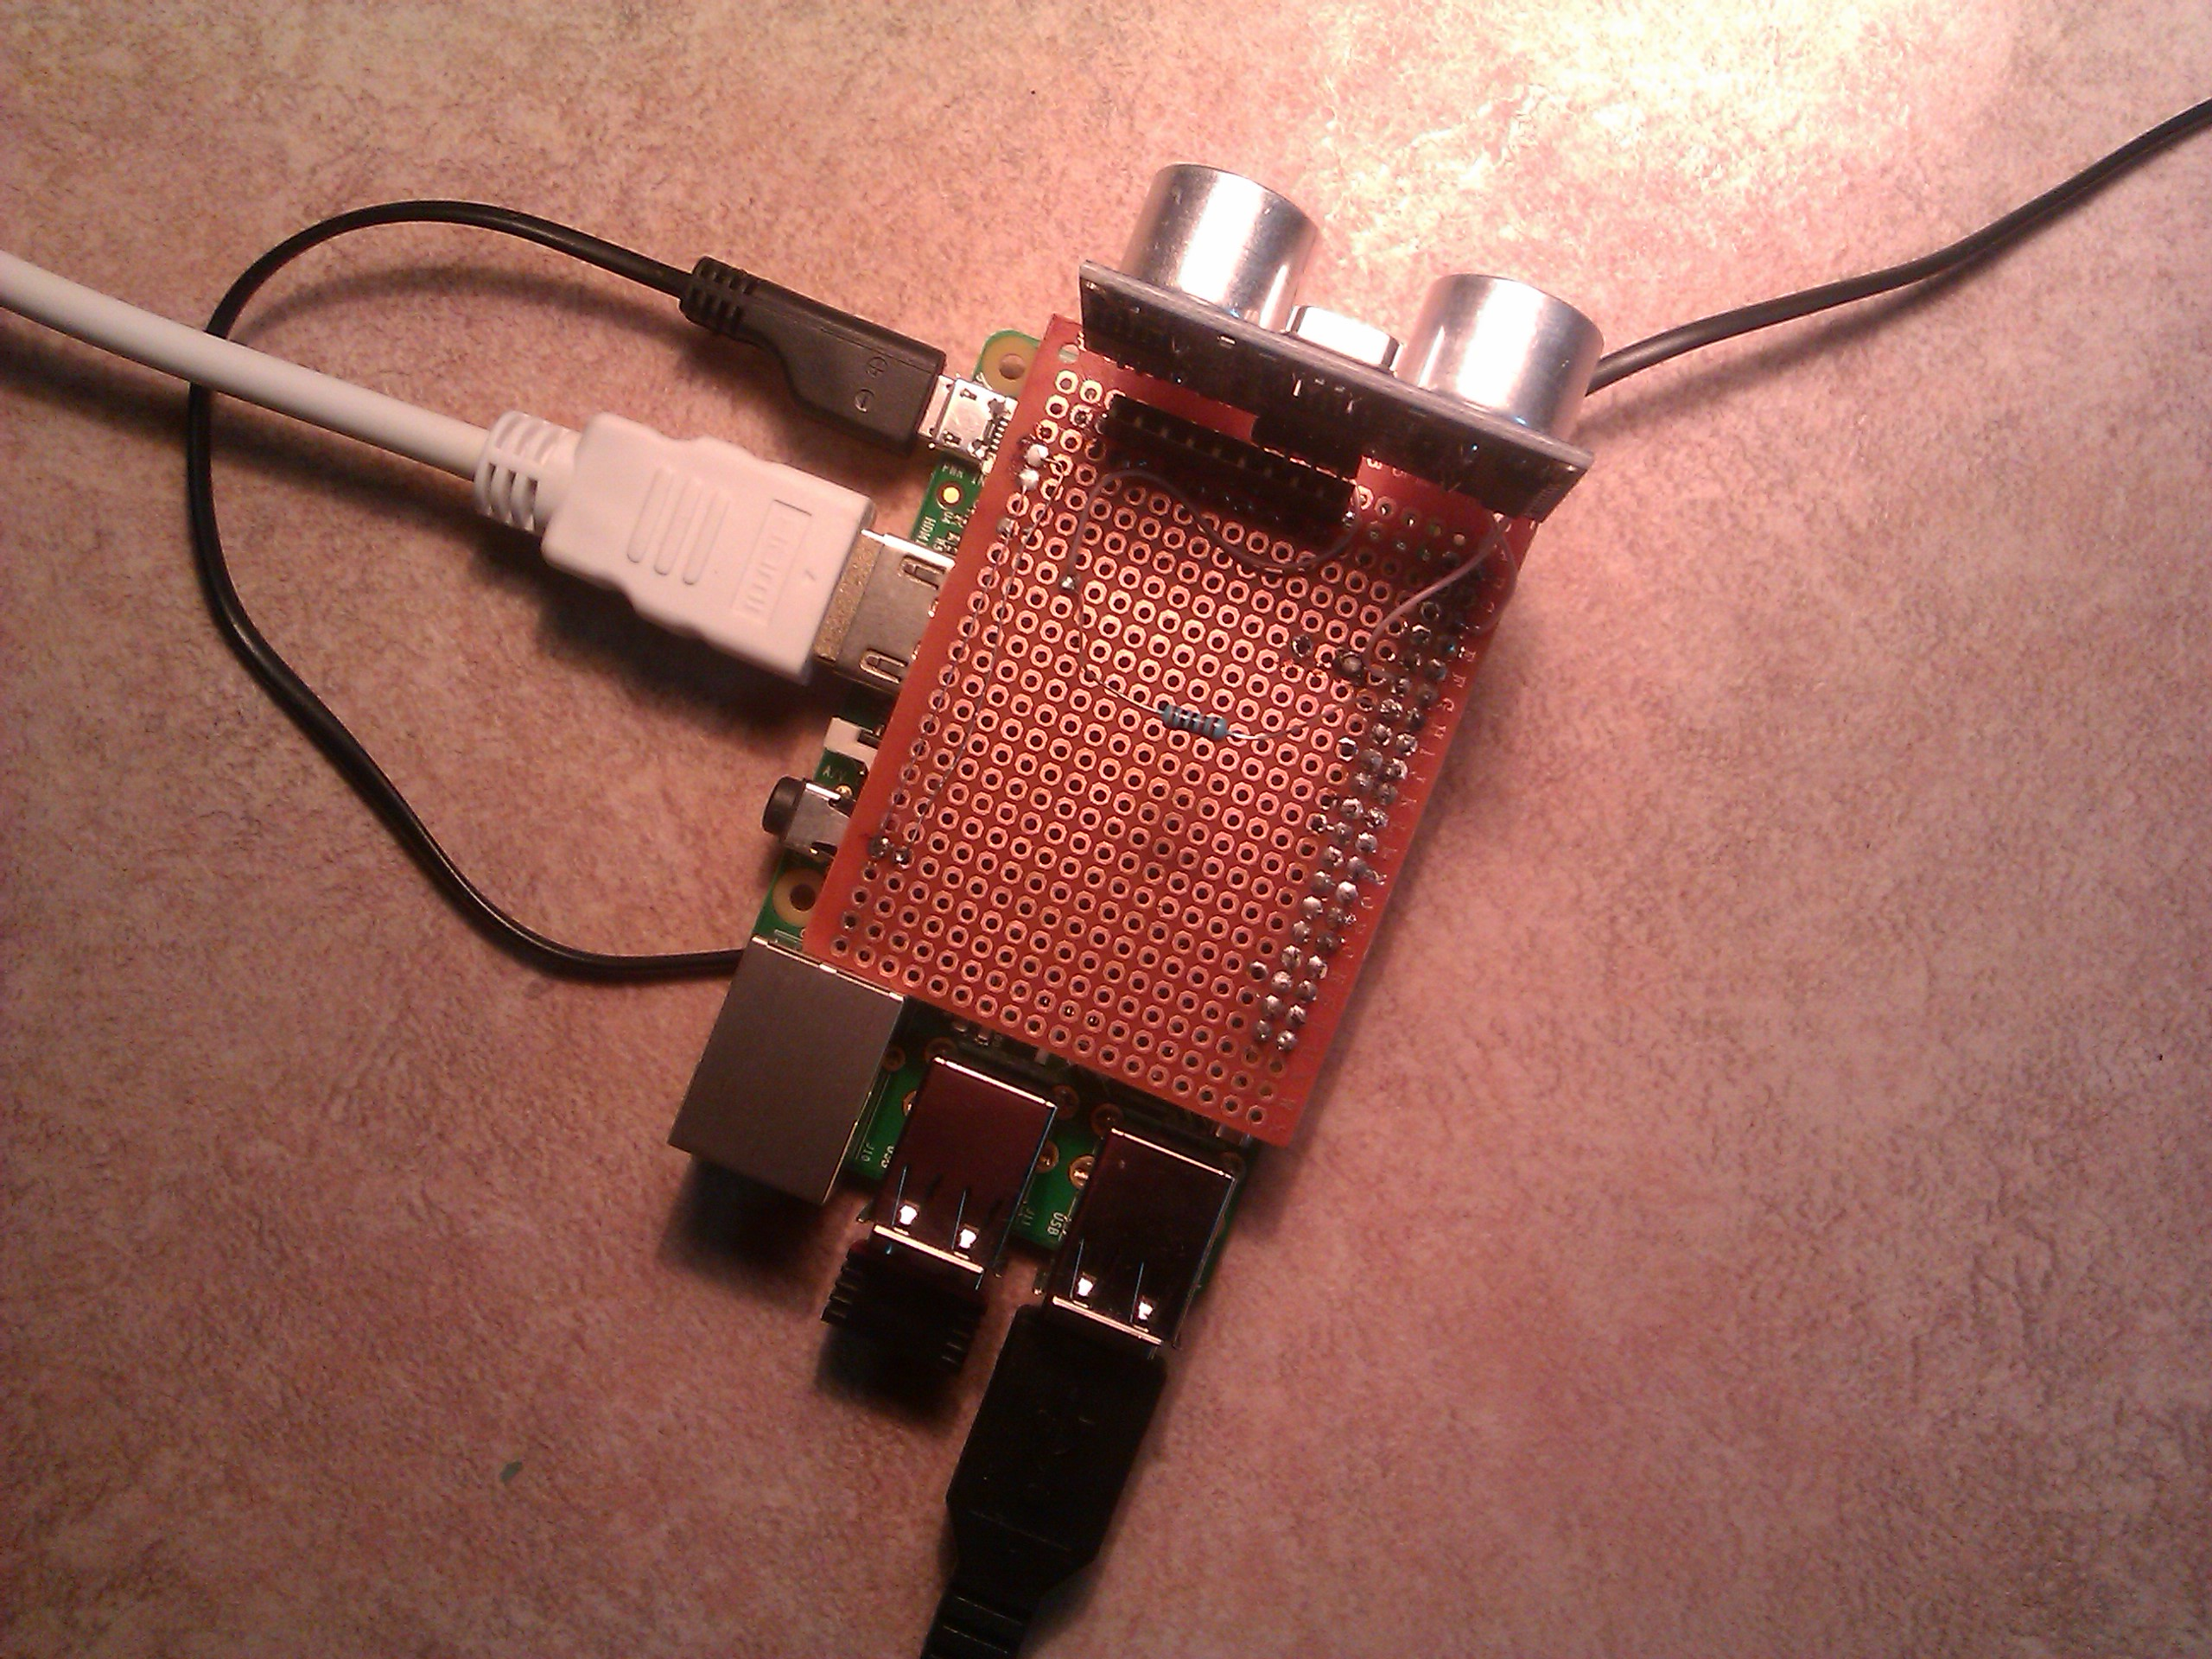
\includegraphics[width=.7\linewidth]{./graphics/raspberry-pi.jpg}
  \end{figure}
\end{frame}

\begin{frame}[label=sec-2-2-4]{А также \ldots}
  \ldots креативное использование ресурсов хакерспейса сотрудниками
  колледжа
  \begin{figure}
    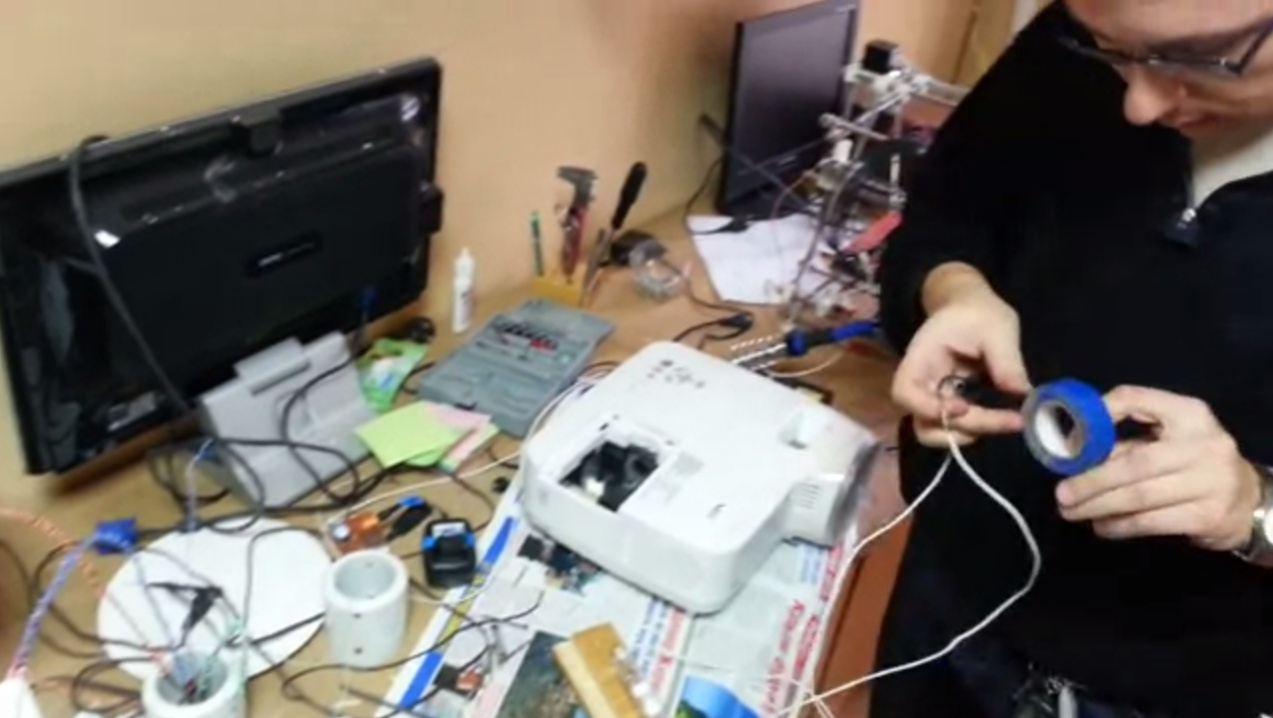
\includegraphics[width=.9\linewidth]{cadr-projector-test}
  \end{figure}
\end{frame}

\begin{frame}[label=sec-2-2-5]{Как стать участником?}
  \begin{enumerate}
  \item Договариваетесь о встрече с администраторами CADR'а --
    предпочтительным способом связи является почтовая рассылка:
    \textbf{cadr-hackerspace@googlegroups.com}
  \item Предоставляете свои контактные данные.
  \item Посещаете несколько встреч.
  \end{enumerate}
\end{frame}

\section{Заключение}
\label{sec-3}
\subsection{Заключение}
\label{sec-3-1}

\begin{frame}[label=sec-3-1-1]{Заключение}
  Информация о хакерспейсе CADR:
  \begin{itemize}
  \item cadrspace.ru
  \item vk.com/cadrspace
  \end{itemize}

  Мои контакты:
  \begin{itemize}
  \item poptsov.artyom@gmail.com \\
    GPG ключ: 0x0898A02F, pgp.mit.edu
  \end{itemize}
\end{frame}

\begin{frame}[label=sec-3-1-2]{Спасибо за внимание!}
  \begin{columns}
    \begin{column}{0.5\textwidth}
      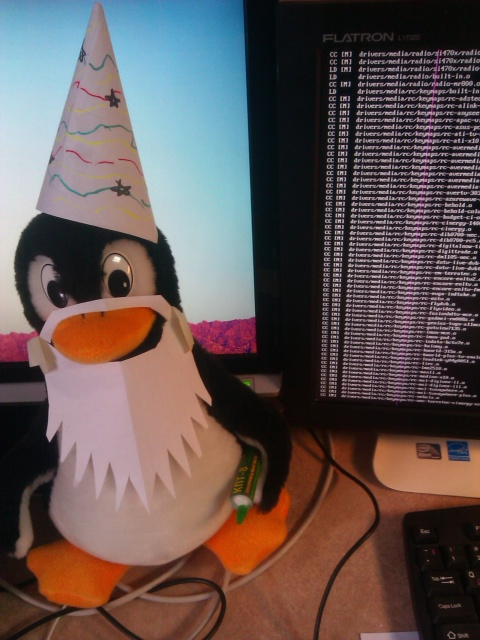
\includegraphics[width=.9\linewidth]{./graphics/tux.jpg}
    \end{column}
  \end{columns}
\end{frame}

\end{document}
